% Asset ID: A21ParametricEquationsTikZ-004
% Source: Transcript sketching section; CCEA A21-CG-LO001.
% Related lesson section: Core Theory; Sketching Parametric Curves.
% Purpose: Show sketching using a table of parameter values.

\documentclass[tikz,border=8pt]{standalone}
\usepackage{amsmath}
\usepackage{pgfplots}
\pgfplotsset{compat=1.18}
\begin{document}
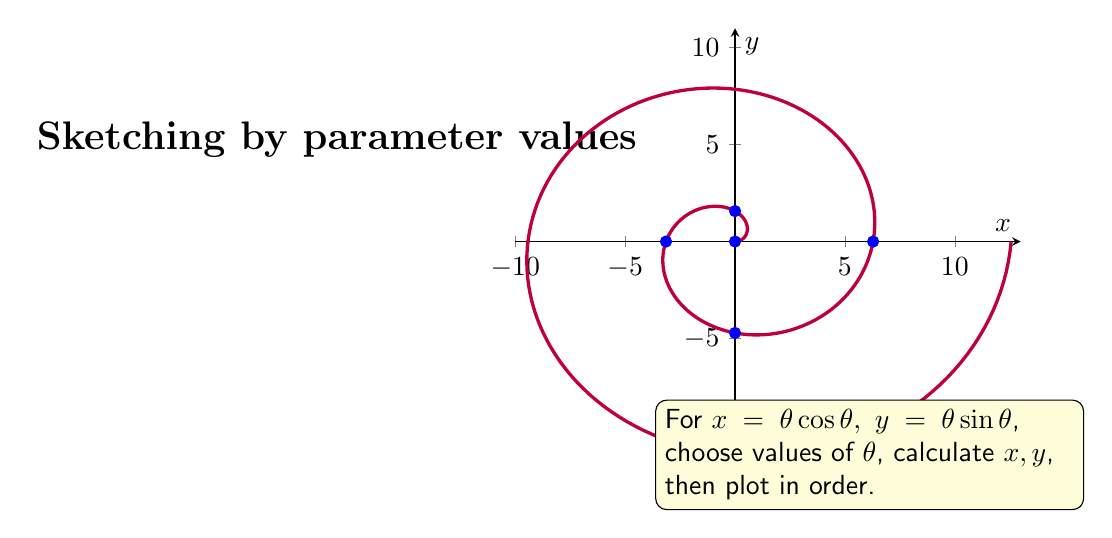
\begin{tikzpicture}[font=\sffamily]

\node[anchor=west, font=\bfseries\Large] at (-6.2,4.0) {Sketching by parameter values};
\begin{axis}[width=8cm,height=7cm,axis lines=middle,xmin=-10,xmax=13,ymin=-11,ymax=11,xlabel={$x$},ylabel={$y$}]
\addplot[domain=0:720,samples=300,purple,very thick] ({x/57.2958*cos(x)},{x/57.2958*sin(x)});
\addplot[only marks,blue] coordinates {(0,0) (0,1.5708) (-3.1416,0) (0,-4.7124) (6.2832,0)};
\end{axis}
\node[draw, rounded corners, fill=yellow!15, text width=5.2cm] at (4.5,0) {For \(x=\theta\cos\theta,\ y=\theta\sin\theta\), choose values of \(\theta\), calculate \(x,y\), then plot in order.};

\end{tikzpicture}
\end{document}
